\lstinputlisting[language=bash,basicstyle=\small]{python_codes/fieldstone_65/keywords.ascii}

\begin{center}
Code at \url{https://github.com/cedrict/fieldstone/tree/master/python_codes/fieldstone_65}
\end{center}

\par\noindent\rule{\textwidth}{0.4pt}
%%%%%%%%%%%%%%%%%%%%%%%%%%%%%%%%%%%%%%%%%%%%%%%%%%%%%%%%%%%%%%%%%%%%%%%%%%%%%%%%%%%%%%%%%%%%

Let us start by remembering that the Peclet number is given by 
\[
\Penb = \frac{uh}{2\kappa} = \frac{uh\rho C_p}{2 k}
\]
where $u$ is the velocity, $h$ is the element size and $\kappa$ is the diffusion coefficient.

%----------------------------
\subsection*{Experiment 1}
We wish to solve the advection-diffusion problem presented in 
Section~\ref{MMM-ss:advdiff}:
\begin{equation}
\rho C_p u \frac{dT}{dx} - k \frac{d^2T}{dx^2} = f \qquad \text{in} \quad [0,L_x]
\end{equation}
with the boundary conditions $T(x=0)=0$ and $T(x=L_x)=0$.

The domain is characterised by $L_x=1$, and since $L_y$ is irrelevant it is set to $L_x/10$.
We further set $nelx=10$, $f=1$, $\rho=1$, $C_p=1$, $u=1$.
We will consider three values of the Peclet number: 0.25, 1 and 5.
From these values we can compute the corresponding heat conductivity value $k$.
Linear elements are used.

The analytical solution is given by Eq.~(2.23) in Donea \& Huerta \cite{dohu03}:
\[
T(x)= \frac{f}{u_0} \left(  x - \frac{1-\exp(2x \; \Penb /h_x)}{1-\exp(2\; \Penb / h_x)} \right) 
\]

As $\Penb$ increases, a sharp gradient, sometimes called a boundary layer,
develops at the right end of the domain. For high $\Penb$ values, the solution shows 
spurious node to node oscillations, failing to capture the highly nonlinear change. This oscillatory
behavior is seen for $\Penb>1$ (see Donea \& Huerta \cite{dohu03}).

\begin{center}
\includegraphics[width=5.5cm]{python_codes/fieldstone_65/results/exp1/solution1.pdf}
\includegraphics[width=5.5cm]{python_codes/fieldstone_65/results/exp1/solution2.pdf}
\includegraphics[width=5.5cm]{python_codes/fieldstone_65/results/exp1/solution3.pdf}\\
\includegraphics[width=5.5cm]{python_codes/fieldstone_65/results/exp1/T1.pdf}
\includegraphics[width=5.5cm]{python_codes/fieldstone_65/results/exp1/T2.pdf}
\includegraphics[width=5.5cm]{python_codes/fieldstone_65/results/exp1/T3.pdf}\\
{\captionfont Left to right: $\Penb$=0.25, $Pe$=1, $Pe$=5}
\end{center}

Finally we see that we recover identical results as in Donea \& Huerta \cite{dohu03}:

\begin{center}
\includegraphics[width=8.6cm]{python_codes/fieldstone_65/images/dohu}
\end{center}

If we now use the artificial diffusion presented in Section~\ref{MMM-ss:supg}, we have
\[
\tilde{\kappa}=\beta \kappa \Penb = \beta \frac{k}{\rho C_p} \Penb
\]
with 
\[
\beta=\coth(\Penb)-\frac{1}{\Penb}
\]
which yields:
\[
\tilde{k} = \tilde{\kappa} \rho_0 C_p 
\]
and the code solves the following equation
\begin{equation}
\rho C_p u \frac{dT}{dx} - (k + \tilde{k})\frac{d^2T}{dx^2} = f \qquad \text{in} \quad [0,L_x]
\end{equation}


We observe that this approach recovers the analytical solution exactly:
\begin{center}
\includegraphics[width=5cm]{python_codes/fieldstone_65/results/exp1/artdiff/T1.pdf}
\includegraphics[width=5cm]{python_codes/fieldstone_65/results/exp1/artdiff/T2.pdf}
\includegraphics[width=5cm]{python_codes/fieldstone_65/results/exp1/artdiff/T3.pdf}\\
{\captionfont Left to right: $\Penb$=0.25, $\Penb$=1, $\Penb$=5}
\end{center}

If one now uses 'full upwinding', i.e. $\beta=1$, we see that the scheme is 
overly dissipative (i.e. overly diffusive):

\begin{center}
\includegraphics[width=5cm]{python_codes/fieldstone_65/results/exp1/artdiff1/T1.pdf}
\includegraphics[width=5cm]{python_codes/fieldstone_65/results/exp1/artdiff1/T2.pdf}
\includegraphics[width=5cm]{python_codes/fieldstone_65/results/exp1/artdiff1/T3.pdf}\\
{\captionfont Left to right: $\Penb$=0.25, $\Penb$=1, $\Penb$=5}
\end{center}

\paragraph{Pure diffusion} It is also worth noting that when the velocity $u=0$, then the ODE becomes 
\begin{equation}
- k \frac{d^2T}{dx^2} = f \qquad \text{in} \quad [0,L_x]
\end{equation}
and its solution is 
\[
T(x)=-\frac{k}{k} (\frac{1}{2}x^2 + a x + b)
\]
Using the boundary conditions $T(x=0)=0$ and $T(x=L_x)=0$, we find
\[
b=0
\qquad
a = Lx/2
\]
so the result is the following parabolic profile: 
\[
T(x)=\frac{f}{2k}x(L_x-x)
\]
with 
\[
q(x)=-\frac{dT}{dx} = -\frac{f}{k}x
\]


%..................................................................................
\subsection*{Experiment 2 - advection skew to the mesh}

The domain is a unit square. Resolution is $10\times10$ linear elements. Initial temperature is 
irrelevant since we compute the steady state field. 

\begin{center}
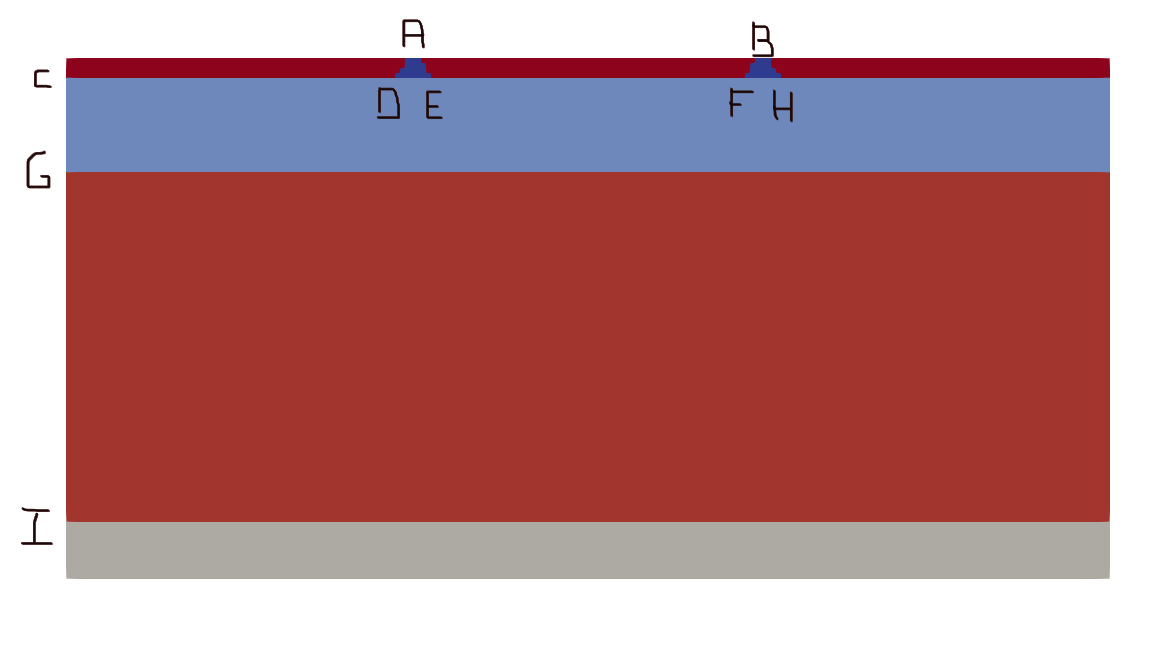
\includegraphics[width=7cm]{python_codes/fieldstone_65/images/setup}
\includegraphics[width=7cm]{python_codes/fieldstone_65/results/exp2/vel}\\
{\captionfont Left: Taken from Donea \& Huerta \cite{dohu03}. In our code we replace $u$ by the 
temperature $T$. Right: prescribed velocity field.}
\end{center}

\begin{remark}
On page 75 of \cite{dohu03} the authors state that 
"the diffusivity coefficient is taken to be $10^{-4}$ , 
corresponding to a mesh Peclet number of $10^4$. 
Given that $\Penb=u h/2\kappa$ and h=0.1, this statement makes no sense.
I have therefore chosen $\Penb=10^4$ and then 
$\kappa=uh/2\Penb = 5\cdot10^{-6}$.
\end{remark}

The norm of the velocity vector $\vec{\upnu}$ is $|\vec{\upnu}|=1$. 
Since the Peclet number is so high, we have 
\[
\tau = \frac{h}{2 u_0} \left( \coth (\Penb) -\frac{1}{\Penb} \right) \rightarrow 
\frac{h}{2 u_0} 
\]

We then conduct three experiments: one without stabilisation, one with (isotropic) artifical diffusion, and 
one with SUPG, from left to right on the following plots:

\begin{center}
\includegraphics[width=15cm]{python_codes/fieldstone_65/results/exp2/Temps2}\\
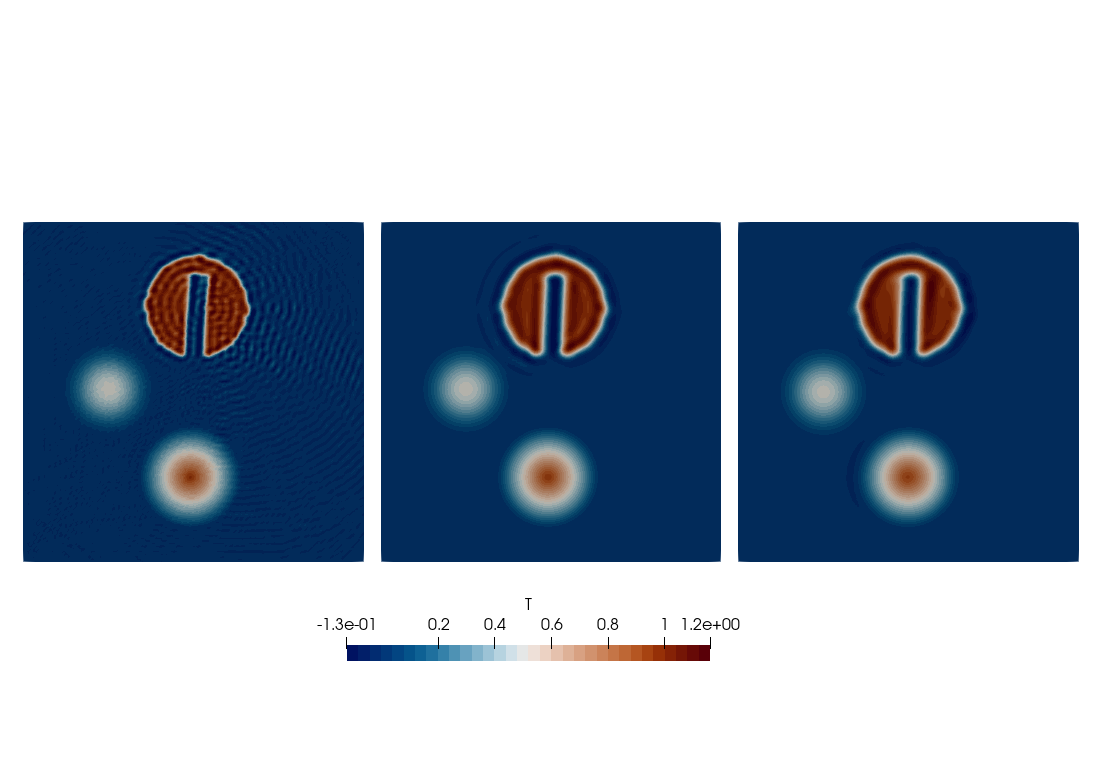
\includegraphics[width=15cm]{python_codes/fieldstone_65/results/exp2/Temps}\\
\includegraphics[width=15cm]{python_codes/fieldstone_65/images/exp2}\\
{\captionfont Left to right: Standard Galerkin method, artificial diffusion, SUPG. 
Bottom row taken from Donea \& Huerta \cite{dohu03}. }
\end{center}



%..................................................................................
\subsection*{Experiment 3 - DG book setup}

This setup comes from Li's book on Discontinuous Galerkin Methods \cite{li06}, Section 5.2.3.
The 2D advection-diffusion equation is solved on a unit square with the following boundary 
conditions:
\begin{itemize}
\item bottom: $T=0$
\item left: $T=0$ if $y>0.5$, $T=1$ otherwise
\item right: $T=0$
\item top: $\partial_y T=0$
\end{itemize} 
Note that is not clear which value is actually prescribed in the lower left corner. 

Coefficients are not specified but the experiment should be run at $u/\kappa=1,10,100$ where 
$D$ is the diffusion coefficient (in the book $D$ is used instead of $\kappa$).
We then set $\rho=C_p=1$, $u_0=1$ and we define $\xi=u/\kappa$ with $\xi=1,10,100$. Then 
\[
\Penb = \frac{h\xi}{2} 
\]
We finally set nelx=nely=32, so that the heat conductivity coefficient can be computed.


\begin{center}
\includegraphics[height=10cm]{python_codes/fieldstone_65/results/exp3/libook}
\includegraphics[height=10cm]{python_codes/fieldstone_65/results/exp3/Tnostab}\\
{\captionfont Left: Taken from Li \cite{li06}. Computed results for a 2-D convection-diffusion 
problem showing the effect of convection on the temperature distribution in the system.
Right: results obtained without any stabilisation. From top to bottom, $\Penb=0.015625$, 
$\Penb=0.15625$ and $\Penb=1.5625$.}
\end{center}

The code also automatically generates the following 3D plots, and we see that for $\xi=100$
we obtain a strong overshoot near the right boundary:

\begin{center}
\includegraphics[width=5cm]{python_codes/fieldstone_65/results/exp3/solution1.pdf}
\includegraphics[width=5cm]{python_codes/fieldstone_65/results/exp3/solution10.pdf}
\includegraphics[width=5cm]{python_codes/fieldstone_65/results/exp3/solution100.pdf}\\
{\captionfont No stabilisation, from left to right: $\xi=1,10,100$.}
\end{center}

If I now increase the resolution then $h$ becomes smaller and so does the Peclet number, so that 
the oscillations near the right wall disappear:

\begin{center}
\includegraphics[width=5cm]{python_codes/fieldstone_65/results/exp3/solution100.pdf}
\includegraphics[width=5cm]{python_codes/fieldstone_65/results/exp3/solution100_x2.pdf}
\includegraphics[width=5cm]{python_codes/fieldstone_65/results/exp3/solution100_x4.pdf}\\
{\captionfont No stabilisation. $\xi=100$. From left to right: 32x32, 64x64 and 128x128 resolution.}
\end{center}

ToDo: run this experiment with SUPG.

%..................................................................................
\subsection*{Experiment 4 - Heat flow around a cylinder} 

This experiment is described in Section~\ref{MMM-sec:hfcyl}.
We vary the Peclet number from $10^{-3}$ to $10^2$. 
The prescribed velocity field is as follows:

\begin{center}
\includegraphics[width=5cm]{python_codes/fieldstone_65/results/exp4/vel}
\end{center}

Zero temperature is prescribed at the bottom and top boundaries.
The steady state temperature fields for $\Penb=0.001, 0.01, 0.1, 1, 10$ 
on a 250x100 grid are shown here:

\begin{center}
\includegraphics[width=5cm]{python_codes/fieldstone_65/results/exp4/temps}
\end{center}

Note that the velocity is not tangential to the bottom and top walls, so that we actually 
prescribe a tempetature on outflow regions, which is not possible! 


